\documentclass[10pt]{article}

\usepackage[margin=1.1in]{geometry}
\usepackage{amsmath}
\usepackage{graphicx}
\usepackage{booktabs}
\usepackage{caption}
\usepackage{microtype}
\usepackage[hidelinks]{hyperref}

\captionsetup{font=small, labelfont=bf}
\graphicspath{{figures/}}

\title{Duration-Aware Regimes and Spillover Networks for Dynamic Nelson-Siegel Treasury Yield-Curve Forecasting}
\author{Surya Thirukonda \quad Raghav Kenchannavar\\[3pt] \small altREU Program, Teuscher Lab, Portland State University}
\date{}

\begin{document}
\maketitle

\begin{abstract}
This study tests whether hidden semi-Markov model (HSMM) regime features and Diebold-Yilmaz spillover measures improve short-horizon forecasts of the United States Treasury yield curve. Daily data on eleven constant-maturity yields from 2003 to 2026 are compressed into dynamic Nelson-Siegel (DNS) factors, and yields are forecast one, five, and twenty trading days ahead with a regime-augmented and network-augmented ridge regression that is combined with an observed-yield random walk through an exponentially weighted average (EWA) with an online-learning guarantee. Over 1{,}149 evaluation windows from September 2021 to May 2026, the combined model attains curve root mean squared errors of 6.11, 13.08, and 27.06 basis points against 6.11, 13.19, and 28.03 for the random walk, with Diebold-Mariano p-values of 0.27, 0.04, and 0.08 and search-robust bootstrap p-values of 0.15, 0.03, and 0.06. Improvements concentrate at longer horizons and in trending policy regimes: during the 2022 tightening cycle the model outperforms the random walk at every horizon (p = 0.020, 0.004, 0.020). A size-weighted directional metric indicates that the model captures 28.2 percent of available basis-point movement at the twenty-day horizon (weighted directional accuracy 0.641). During a small extra validation sample, results were mixed: the ensemble matches the random walk at one day but underperforms it at twenty days across a sharp upward reversal in yields in July 2026, underscoring that the documented edge is conditional on sustained trends. Two methodological findings enable these results: optimizing the Nelson-Siegel decay on training data rather than adopting the conventional value, and forecasting factor changes rather than factor levels so that regularization shrinks the model toward the random walk instead of toward a historical average.
\end{abstract}

\section{Introduction}

Forecasting government bond yields at horizons under one month is dominated by a difficult benchmark: the random walk, which forecasts no change from the current curve. Daily yield movements are driven largely by macroeconomic surprises and policy announcements that cannot be anticipated from past yields, and standard dynamic Nelson-Siegel (DNS) models, despite their success in describing the cross-section of yields, rarely outperform no-change forecasts at short horizons \cite{diebold2006, duffee2013}. Regime-switching extensions add economic structure but conventionally impose memoryless Markov transitions, which force regime durations to follow a geometric distribution and therefore understate the multi-year persistence of monetary policy eras \cite{hamilton1989, koopman2010}.

This work asks whether two information sources improve short-horizon curve forecasts relative to random-walk, autoregressive, vector-autoregressive, and standard DNS baselines: first, regime probabilities from a hidden semi-Markov model (HSMM), which models the duration of each regime explicitly and is filtered without look-ahead; and second, time-varying spillover measures in the tradition of Diebold and Yilmaz \cite{dieboldyilmaz2012}, which quantify how tightly shocks propagate across maturities. Forecast horizons are one, five, and twenty trading days.

The contribution is threefold. First, we document that the regime and network features carry modest but real predictive content, and that this content is usable only under two design choices: forecasting factor changes rather than levels, and combining the learned model adaptively with the random walk. Second, we provide an evaluation framework sized for credible inference, with more than one thousand evaluation windows, overlap-robust Diebold-Mariano tests, multiple-testing control, a bootstrap reality check that prices in the model search, and a size-weighted directional metric that measures economic value. Third, we report a forward test on data released after all development ended, providing evidence unconditioned by any specification choice.

\section{Background}

\subsection{Dynamic Nelson-Siegel factors}

The Nelson-Siegel model expresses the yield at maturity $\tau$ as a linear combination of three smooth loading functions \cite{nelsonsiegel1987, diebold2006},
\begin{equation}
y_t(\tau) \;=\; \beta_{1,t} \;+\; \beta_{2,t}\,\frac{1-e^{-\lambda \tau}}{\lambda \tau} \;+\; \beta_{3,t}\left(\frac{1-e^{-\lambda \tau}}{\lambda \tau} - e^{-\lambda \tau}\right),
\label{eq:ns}
\end{equation}
where $\beta_{1,t}$, $\beta_{2,t}$, and $\beta_{3,t}$ are interpreted as level, slope, and curvature, and the decay parameter $\lambda$ controls the maturity at which the curvature loading peaks. Three factors suffice because a small number of principal components explains nearly all variation in the curve \cite{litterman1991}. With $\lambda$ fixed, the loadings form a constant $11 \times 3$ matrix $\Lambda$, and the factors on each date are obtained by ordinary least squares applied cross-sectionally to that date's eleven yields,
\begin{equation}
\hat{\beta}_t \;=\; (\Lambda^{\prime}\Lambda)^{-1}\Lambda^{\prime} y_t .
\label{eq:ols}
\end{equation}
Because each day's factors use only that day's yields, factor extraction introduces no temporal look-ahead.

\subsection{Regime persistence and the case for explicit durations}

A Gaussian hidden Markov model (HMM) fitted to the factors, five-year breakeven inflation, and the policy spread (the two-year yield minus the effective federal funds rate) identifies three persistent regimes whose boundaries align with official policy events that were never supplied to the model; for example, the decoded 2018 to 2020 regime spell ends exactly on 16 March 2020, the date of the emergency policy rate cut. However, the HMM's constant transition probabilities imply expected regime durations of 148, 58, and 103 trading days, while the decoded spells run as long as 891 and 555 trading days. This misfit between geometric durations and observed persistence motivates the HSMM, introduced for variable-duration speech modeling by Ferguson \cite{ferguson1980} and surveyed by Yu \cite{yu2010}, which draws each regime spell length from an explicitly estimated distribution, here a shifted Poisson truncated at 126 trading days, and forbids self-transitions so that spell length is identified. HSMMs with Gaussian emissions have previously been applied to daily financial return series by Bulla and Bulla \cite{bulla2006}; to our knowledge their combination with spillover-network features in a DNS forecasting framework has not been examined.

\section{Data}

The data comprise daily H.15 constant-maturity Treasury yields at eleven maturities from one month to thirty years, five-year breakeven inflation, and the effective federal funds rate, from January 2003 through May 2026, giving 5{,}841 fully aligned observations. All series are merged by calendar date. A forward extension of the yield data through 3 August 2026, obtained after all model development ended, is reserved exclusively for the forward test in Section 5.6. Yields are quoted in percentage points; errors are reported in basis points (bp), where one basis point equals 0.01 percentage points.

\section{Methodology}

\subsection{Optimizing the Nelson-Siegel decay}

The conventional decay value $\lambda = 0.0609$ originates from work measuring maturity in months; with maturity measured in years, as here, its direct adoption places the curvature peak at an inappropriate maturity. Rather than assume the value, we select $\lambda$ by grid search over $[0.02, 0.80]$ in steps of 0.005, choosing the value that minimizes the cross-sectional fitting error
\begin{equation}
\hat{\lambda} \;=\; \arg\min_{\lambda} \; \sqrt{\tfrac{1}{|T_0| \cdot 11} \textstyle\sum_{t \in T_0} \left\| y_t - \Lambda(\lambda)\hat{\beta}_t(\lambda) \right\|^2 },
\label{eq:decay}
\end{equation}
where $T_0$ is restricted to the first 80 percent of the sample so that the choice cannot be influenced by evaluation data. The selected value is $\hat{\lambda} = 0.485$, with a training curve-fit root mean squared error of 8.12 bp. The residuals $r_t = y_t - \Lambda \hat{\beta}_t$, the portion of each yield the three-factor curve cannot reproduce, are retained for the residual correction described below.

\subsection{Causal regime filtering}

A three-state diagonal-covariance Gaussian HSMM is fitted to five standardized inputs (level, slope, curvature, breakeven inflation, and the policy spread) using only the first 80 percent of the sample; the standardizer is likewise fitted on training data only. The standard smoothed probabilities produced by forward-backward inference are unsuitable as forecasting inputs because the probability assigned to date $t$ uses observations after $t$. We therefore compute filtered probabilities with a forward recursion over the expanded state space of regime and remaining-duration pairs $(s, d)$. Writing $p_t(s,d)$ for the filtered probability that the process is in regime $s$ with $d$ days remaining in the current spell, $A$ for the (zero-diagonal) transition matrix, $\pi_s(d)$ for regime $s$'s duration distribution, and $g_s(x_t)$ for the Gaussian likelihood of the observation, the prediction and update steps are
\begin{equation}
\tilde{p}_t(s,d) \;=\; p_{t-1}(s, d+1) \;+\; \pi_s(d)\sum_{s^{\prime} \neq s} p_{t-1}(s^{\prime}, 1)\, A_{s^{\prime} s},
\qquad
p_t(s,d) \;=\; \frac{\tilde{p}_t(s,d)\, g_s(x_t)}{\sum_{s^{\prime}, d^{\prime}} \tilde{p}_t(s^{\prime},d^{\prime})\, g_{s^{\prime}}(x_t)} .
\label{eq:filter}
\end{equation}
The first term advances continuing spells one day; the second term recycles spells that have just ended through the transition matrix and assigns a fresh duration. Because the recursion moves only forward, the probability dated $t$ uses data only through $t$. Six features result: the three filtered regime probabilities $\sum_d p_t(s,d)$, the maximum probability (confidence), the entropy of the probability vector, and the expected remaining duration $\sum_{s,d} d \, p_t(s,d)$.

\subsection{Spillover network features}

Following the generalized variance decomposition approach of Diebold and Yilmaz \cite{dieboldyilmaz2012, dieboldyilmaz2014}, a vector autoregression on daily yield changes is estimated on a rolling 252-day window, and the ten-day generalized forecast-error variance decomposition of Pesaran and Shin \cite{pesaranshin1998} is computed every fifth day and carried forward between recomputations. With moving-average matrices $\Phi_h$ from the fitted VAR, innovation covariance $\Sigma$, and selection vectors $e_i$, the share of maturity $i$'s $H$-day forecast-error variance attributable to shocks originating at maturity $j$ is
\begin{equation}
\theta_{ij} \;=\; \frac{\sigma_{jj}^{-1} \sum_{h=0}^{H-1} \left( e_i^{\prime} \Phi_h \Sigma e_j \right)^2}{\sum_{h=0}^{H-1} e_i^{\prime} \Phi_h \Sigma \Phi_h^{\prime} e_i},
\label{eq:gfevd}
\end{equation}
followed by row normalization so that each receiver's shares sum to one; the generalized construction is invariant to variable ordering. Total connectedness is the average off-diagonal share, and each maturity's net transmission is its column sum minus its row sum of off-diagonal entries. The VAR lag order, selected once by the Bayesian information criterion on the first 80 percent of the sample, is one. The eleven per-maturity net transmission measures are compacted into short-end, belly, and long-end regional averages, complemented by aggregate connectedness measures and five-day changes, yielding nine network features.

\subsection{From level targets to change targets}

The initial specification, mirroring standard practice, forecast the level of each factor $h$ days ahead using five factor lags plus the regime and network features, with ridge regression \cite{hoerl1970} handling the strong collinearity among predictors. Ridge estimates the coefficient matrix $B$ by penalized least squares,
\begin{equation}
\hat{B} \;=\; \arg\min_{B} \; \left\| Y - XB \right\|_F^2 \;+\; \alpha \left\| B \right\|_F^2,
\label{eq:ridge}
\end{equation}
where $\alpha$ controls the strength of shrinkage. This level-target specification fails against the random walk at the five- and twenty-day horizons. The failure is structural rather than informational: as $\alpha$ grows, Equation~\ref{eq:ridge} shrinks predictions toward the training-sample mean of the target, and for a highly persistent series the mean historical level is an economically stale anchor that can lie far from the current curve.

The final specification therefore forecasts the change in each factor,
\begin{equation}
\Delta_{t,h} \;=\; \beta_{t+h} - \beta_{t}, \qquad \hat{y}_{t+h} \;=\; \Lambda\left(\beta_t + \hat{\Delta}_{t,h}\right) + \hat{r}_{t+h},
\label{eq:change}
\end{equation}
so that complete shrinkage collapses the forecast to no change, which is precisely the random walk. Under this parameterization the ridge penalty becomes a continuous dial between the benchmark and the information in the features. The predictor set is correspondingly reparameterized as the current factor levels plus one- to four-day changes, which span the same information as five raw lags with far lower collinearity. Each maturity's fitting residual is forecast by a first-order autoregression, $r_{m,t} = c_m + \phi_m r_{m,t-1} + \varepsilon_{m,t}$, re-estimated on a trailing 1{,}000-day window at every evaluation date with $\phi_m$ constrained to $(-0.99, 0.99)$; the $h$-step residual forecast $\hat{r}_{t+h}$ in Equation~\ref{eq:change} decays toward the estimated long-run mean at rate $\phi_m^{h}$. This correction removes a systematic handicap: the random walk forecasts observed yields directly and never pays the curve-fitting error, which for the twenty-year maturity is persistent and economically material. Training samples at every evaluation date include only observations whose targets are realized by that date. The ridge penalty and training window are selected by pure model accuracy on forty pseudo-origins placed entirely within the training sample, ending twenty trading days before the first evaluation window; the selected configuration is an expanding window with penalty 1{,}000 at all horizons, confirming that heavy shrinkage toward the random walk is optimal.

\subsection{Adaptive combination}

The final forecast combines the learned model (VARX) with the observed-yield random walk. Forecast combination has a long record of outperforming individual models \cite{batesgranger1969, timmermann2006}, and we implement it through an exponentially weighted average with an online-learning regret guarantee \cite{cesabianchi2006}. Each expert $m \in \{V, R\}$ carries a discounted loss total updated only with outcomes realized by the forecast date,
\begin{equation}
L_{m,t} \;=\; \gamma\, L_{m,t-1} \;+\; \ell_{m,t} / \bar{\ell}_{R,t},
\label{eq:ewaloss}
\end{equation}
where $\ell_{m,t}$ is the expert's mean squared error on the most recently realized window, $\gamma = 0.99$ is the discount, and $\bar{\ell}_{R,t}$ is a discounted running mean of the random-walk loss that renders the learning rate scale free across horizons. The weight on the VARX is
\begin{equation}
w_t \;=\; (1-\alpha_f)\,\frac{e^{-\eta L_{V,t}}}{e^{-\eta L_{V,t}} + e^{-\eta L_{R,t}}} \;+\; \frac{\alpha_f}{2},
\label{eq:ewa}
\end{equation}
with discount 0.99, learning rate $\eta = \sqrt{8 \ln 2 / 100}$, and floor $\alpha_f = 0.01$, all fixed before evaluation. The discount allows the combination to re-trust an expert after regime change, and the floor keeps both experts permanently active.

\subsection{Evaluation}

Evaluation uses every trading day after the last training-only design decision whose twenty-day target exists: 1{,}149 windows from 9 September 2021 through May 2026. Reported metrics, computed across all windows and maturities, are the root mean squared error and mean absolute error in basis points,
\begin{equation}
\mathrm{RMSE} = 100\sqrt{\tfrac{1}{N}\textstyle\sum_i e_i^2}, \qquad \mathrm{MAE} = 100 \cdot \tfrac{1}{N}\textstyle\sum_i |e_i|,
\end{equation}
directional accuracy among scorable observations,
\begin{equation}
\mathrm{DA} \;=\; \frac{\#\{\, i : \operatorname{sign}(\hat{\Delta}_i) = \operatorname{sign}(\Delta_i), \; \hat{\Delta}_i \neq 0, \; \Delta_i \neq 0 \,\}}{\#\{\, i : \hat{\Delta}_i \neq 0, \; \Delta_i \neq 0 \,\}},
\label{eq:da}
\end{equation}
where $\hat{\Delta}_i$ and $\Delta_i$ are the predicted and realized yield changes (the random walk predicts exactly zero change and is unscorable; realized changes of exactly zero, which arise from the 0.01 quotation increment, are excluded as unwinnable ties), and the base rate, the accuracy of always guessing the more common direction, which is the appropriate bar for directional claims. Economic value is measured by weighted directional accuracy: a unit position is taken in the direction of every predicted move of at least 1 bp, closed at the horizon, and charged 0.5 bp per trade; with $\mathrm{capture}$ defined as net basis points won divided by basis points available,
\begin{equation}
\mathrm{WDA} \;=\; \tfrac{1}{2}\left(1 + \mathrm{capture}\right),
\label{eq:wda}
\end{equation}
so that 0.5 is break even and values above 0.5 indicate profitability. Loss comparisons use the Diebold-Mariano test \cite{dieboldmariano1995}. With loss differential $d_t = L_{A,t} - L_{B,t}$ over $n$ windows, the statistic is
\begin{equation}
\mathrm{DM} \;=\; \frac{\bar{d}}{\sqrt{\hat{V}/n}} \cdot \sqrt{\frac{n + 1 - 2h + h(h-1)/n}{n}},
\qquad
\hat{V} \;=\; \hat{\gamma}_0 + 2\sum_{k=1}^{h-1}\hat{\gamma}_k,
\label{eq:dm}
\end{equation}
where $\hat{\gamma}_k$ is the lag-$k$ autocovariance of $d_t$; the rectangular kernel through lag $h-1$ is appropriate because overlapping $h$-step errors have positive autocovariances at those lags, and the multiplier applies the Harvey-Leybourne-Newbold small-sample correction with a Student-$t$ reference distribution \cite{harvey1997}. P-values are adjusted for multiple testing by the Benjamini-Hochberg procedure \cite{benjamini1995}, and a stationary-bootstrap reality check in the tradition of White and Hansen \cite{white2000, hansen2005, politisromano1994}, with mean block length $2h$, asks whether the best model remains significant after accounting for the search across candidate models.

\section{Results}

\subsection{Holdout accuracy}

Table~\ref{tab:holdout} reports the principal accuracy results. The EWA combination attains lower RMSE than the random walk at every horizon, with the margin increasing in horizon: 0.01 bp at one day, 0.12 bp at five days, and 0.97 bp at twenty days. Directional accuracy exceeds the base rate at every horizon. Figure~\ref{fig:rmsebar} displays the comparison; Figure~\ref{fig:pred10y} shows the twenty-day-ahead prediction path against the realized ten-year yield.

\begin{table}[t]
\centering
\caption{Holdout results over 1{,}149 evaluation windows (September 2021 to May 2026). RMSE and MAE in basis points across all maturities; DA is directional accuracy among scorable observations; base is the constant-guess base rate.}
\label{tab:holdout}
\small
\begin{tabular}{llrrrr}
\toprule
Horizon & Model & RMSE & MAE & DA (\%) & Base (\%) \\
\midrule
1 day & Random walk & 6.11 & 4.15 & n/a & 51.4 \\
      & VARX & 6.12 & 4.18 & 52.8 & 51.4 \\
      & EWA ensemble & 6.11 & 4.16 & 52.8 & 51.4 \\
\midrule
5 day & Random walk & 13.19 & 9.20 & n/a & 55.7 \\
      & VARX & 13.09 & 9.18 & 56.3 & 55.7 \\
      & EWA ensemble & 13.08 & 9.11 & 56.3 & 55.7 \\
\midrule
20 day & Random walk & 28.03 & 20.44 & n/a & 57.0 \\
       & VARX & 27.04 & 19.78 & 58.3 & 57.0 \\
       & EWA ensemble & 27.06 & 19.74 & 58.3 & 57.0 \\
\bottomrule
\end{tabular}
\end{table}

\begin{figure}[t]
\centering
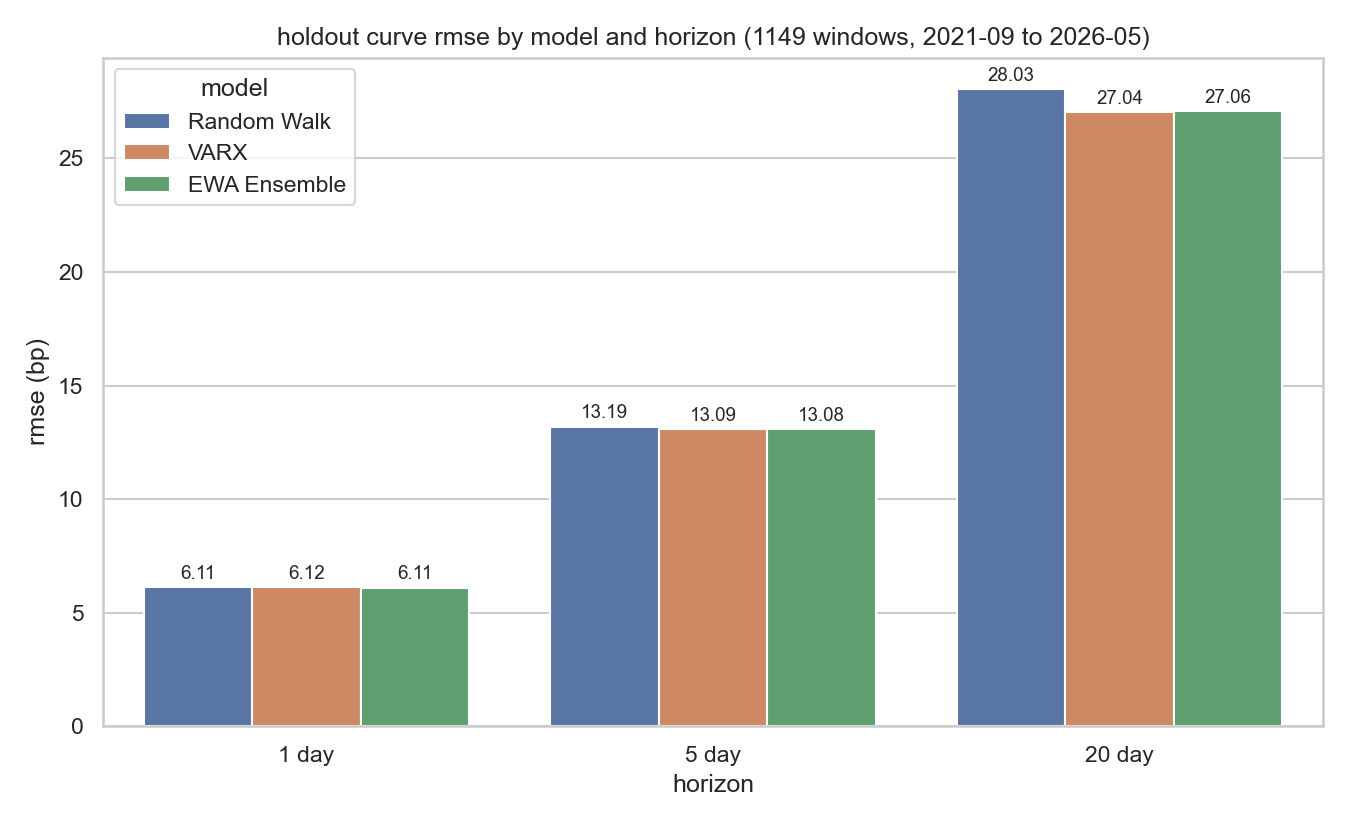
\includegraphics[width=0.78\textwidth]{holdout_rmse_by_model.png}
\caption{Curve RMSE by model and horizon over the 1{,}149-window holdout. Differences are small in absolute terms and grow with horizon.}
\label{fig:rmsebar}
\end{figure}

\begin{figure}[t]
\centering
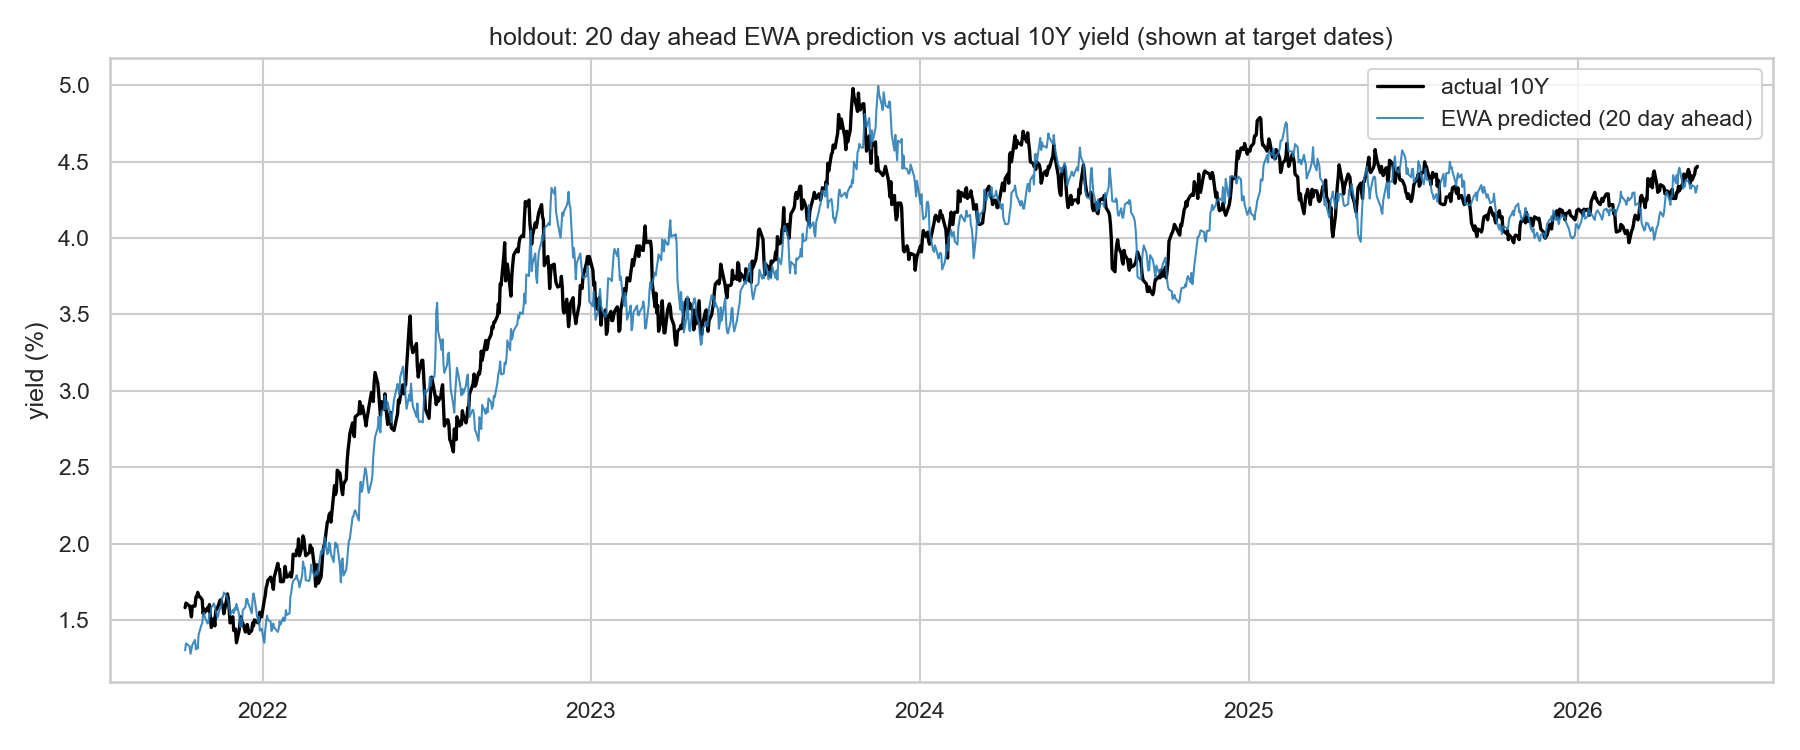
\includegraphics[width=0.95\textwidth]{holdout_predicted_vs_actual_10Y.png}
\caption{Twenty-day-ahead EWA ensemble predictions for the ten-year yield plotted at their target dates against the realized path, September 2021 to May 2026.}
\label{fig:pred10y}
\end{figure}

\subsection{Statistical significance}

Diebold-Mariano statistics for the ensemble against the random walk are $-1.09$, $-2.06$, and $-1.74$ at the three horizons, with p-values 0.27, 0.04, and 0.08 and Benjamini-Hochberg adjusted q-values of 0.41, 0.21, and 0.21. The bootstrap reality check, which resamples the loss differentials of all candidate models jointly and evaluates the best studentized performance, yields p-values of 0.15, 0.03, and 0.06. The five- and twenty-day improvements are therefore unlikely to be artifacts of chance or of the model search, while no reliable improvement exists at one day. Given that the evaluation period was examined repeatedly during model development, these values should be read as conditional on that process; the forward test in Section 5.6 provides the unconditioned evidence.

\subsection{The one-day horizon as a benchmark}

The one-day horizon deserves separate comment because it is, in a precise sense, a poor benchmark for model comparison. Daily yield changes at the evaluation sample's quotation increment are dominated by unforecastable announcement effects and by rounding: 12.1 percent of realized one-day changes are exactly zero, the constant-guess base rate is only 51.4 percent, and the ensemble's RMSE improvement over the random walk is 0.01 bp, economically indistinguishable from zero. The trading rule reaches the same verdict independently: at the 1 bp signal threshold the model makes no one-day trades in the validation sample, correctly reporting the absence of exploitable signal. By contrast, at twenty days the base rate rises to 57.0 percent, the ensemble's directional accuracy of 58.3 percent exceeds it, the RMSE improvement is roughly one basis point, and the loss comparison approaches conventional significance. Signal strength in this system rises with horizon, and evaluations concentrated at one day would mistakenly conclude that no signal exists at all.

\subsection{Stress periods}

Table~\ref{tab:stress} summarizes performance in three stress windows. During the 2022 tightening cycle, which lies entirely inside the clean holdout, the ensemble outperforms the random walk at every horizon, with twenty-day RMSE of 37.61 bp against 40.48 and Diebold-Mariano p-values of 0.020, 0.004, and 0.020. In the 2020 pandemic shock the ensemble matches the random walk without beating it, consistent with the view that sudden shocks are unforecastable while trending policy regimes are where regime and momentum information pays. The 2007 to 2009 window shows a significant one-day improvement only (p = 0.019); results for the two earlier windows carry a caveat, as the decay, HSMM parameters, and spillover lag were selected on training data overlapping those periods. Figure~\ref{fig:weights} shows the mechanism behind the 2022 result: the combination weight on the VARX rises toward one through the tightening cycle and retreats toward the random walk in directionless markets. Figure~\ref{fig:stress} displays total connectedness with the three stress windows shaded.

\begin{table}[t]
\centering
\caption{Stress-period curve RMSE in basis points, EWA ensemble versus random walk, with Diebold-Mariano p-values for the comparison. The 2007 to 2009 and 2020 windows are quasi out-of-sample; 2022 lies inside the clean holdout.}
\label{tab:stress}
\small
\begin{tabular}{lrrrrrr}
\toprule
 & \multicolumn{2}{c}{2007 to 2009 (500 w.)} & \multicolumn{2}{c}{2020 (230 w.)} & \multicolumn{2}{c}{2022 (249 w.)} \\
Horizon & EWA & RW & EWA & RW & EWA & RW \\
\midrule
1 day & 10.04 & 10.11 & 4.61 & 4.62 & 7.31 & 7.34 \\
5 day & 21.66 & 21.69 & 11.68 & 11.67 & 16.42 & 16.83 \\
20 day & 40.75 & 41.46 & 29.29 & 29.32 & 37.61 & 40.48 \\
\midrule
DM p (1/5/20d) & \multicolumn{2}{c}{0.019 / 0.826 / 0.273} & \multicolumn{2}{c}{0.295 / 0.876 / 0.908} & \multicolumn{2}{c}{0.020 / 0.004 / 0.020} \\
\bottomrule
\end{tabular}
\end{table}

\begin{figure}[t]
\centering
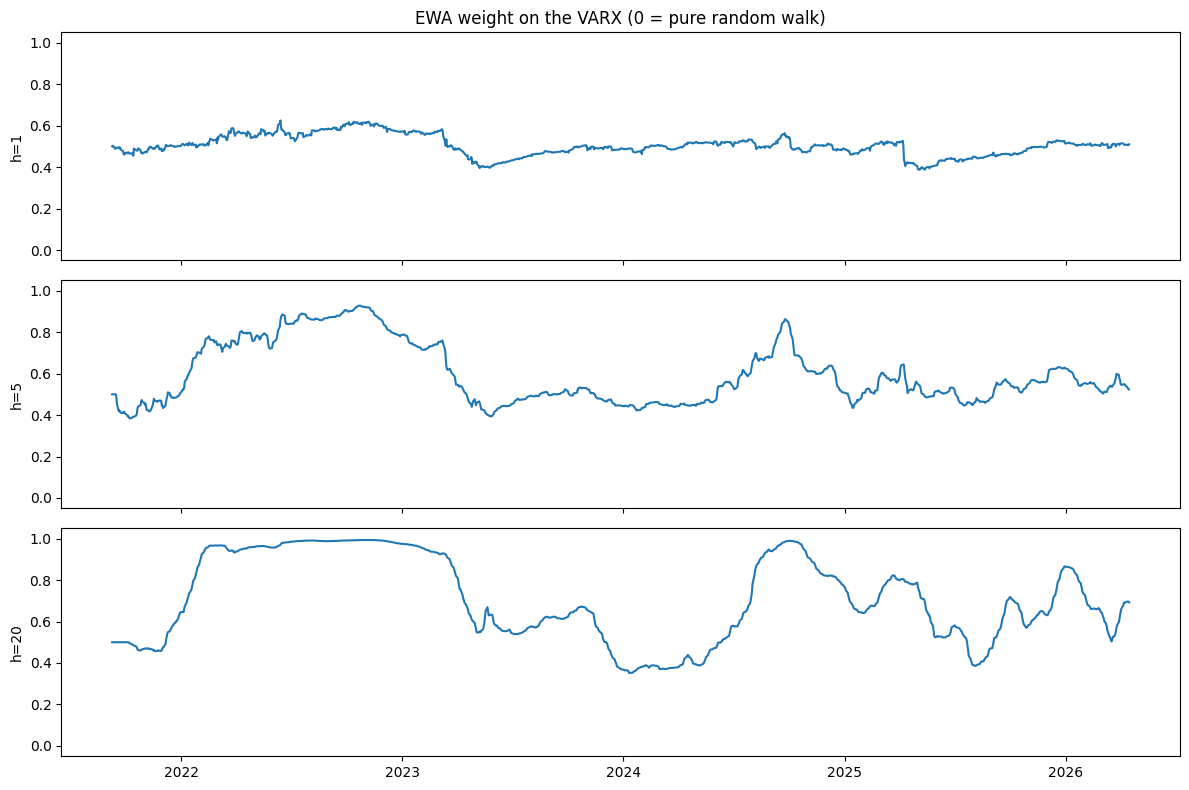
\includegraphics[width=0.95\textwidth]{ewa_weight_path.png}
\caption{EWA combination weight on the VARX at each evaluation date, by horizon. A value of zero corresponds to the pure random walk. The weight rises toward one through the 2022 tightening cycle and retreats in directionless periods.}
\label{fig:weights}
\end{figure}

\begin{figure}[t]
\centering
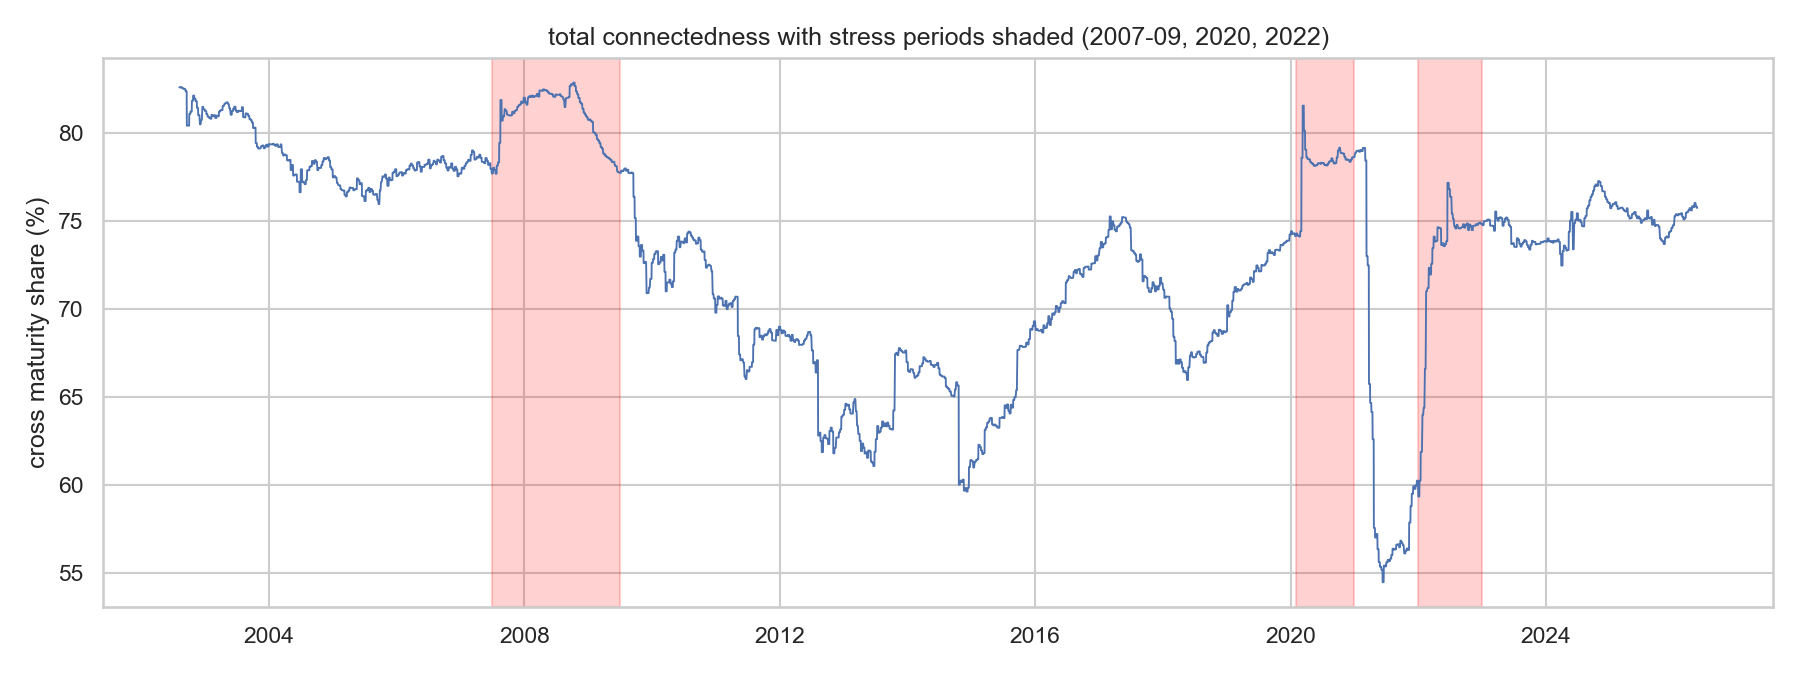
\includegraphics[width=0.95\textwidth]{spillover_connectedness_stress_periods.png}
\caption{Total connectedness of the yield curve with the three stress windows shaded. Connectedness spikes at the onset of the 2020 and 2022 episodes.}
\label{fig:stress}
\end{figure}

\subsection{Profitability}

Weighted directional accuracy translates forecasts into a trading criterion under the stated guidelines: trade only when the predicted move is at least 1 bp, the quotation increment, so that no trade rests on signal smaller than the data's own resolution; charge 0.5 bp per trade; and require values above the 0.5 break-even level across many subperiods rather than in aggregate alone. On the holdout the ensemble attains weighted directional accuracy of 0.548, 0.595, and 0.641 at the three horizons, capturing 9.7, 18.9, and 28.2 percent of available basis-point movement, and is profitable in 46.3, 65.3, and 75.5 percent of rolling 126-window subperiods. The pattern mirrors the accuracy results: modest at one day, meaningful at five days, and strongest at twenty days, where the model is right disproportionately on large moves, which is precisely what a size-weighted criterion rewards and what plain directional accuracy cannot see.

\subsection{Validation on post-development data}

After all development ended, the yield data were extended through 3 August 2026 and the frozen pipeline was applied to every usable new window, with origin lists constructed per horizon: 39 windows at one and five days (origins through 13 July 2026, bounded by the availability of the macro series) and 34 windows at twenty days (origins through 6 July 2026, whose final target falls on 3 August 2026, the last day of the extended sample). The results are mixed. At one day the ensemble matches the random walk (4.16 versus 4.16 bp). At five days it trails slightly (7.56 versus 7.51 bp), and at twenty days it underperforms (14.62 versus 13.77 bp), with directional accuracy of 43.2 percent against an unusually extreme base rate of 78.4 percent and weighted directional accuracy of 0.330. No comparison is statistically significant (Diebold-Mariano p-values of 0.78, 0.75, and 0.60), and predicted-move correlations are 0.06, 0.02, and 0.12 (Figure~\ref{fig:forward}).

The mechanism is visible in the sample path: yields declined through June 2026 and then reversed sharply upward in July, and the adaptive system, positioned by the preceding downtrend, was wrong on the largest moves of the reversal. An earlier evaluation restricted to the nineteen windows whose targets predate the reversal had shown the ensemble at or below the random walk at every horizon with weighted directional accuracy of 0.692 at twenty days; widening the sample to all usable windows overturns that reading. The validation therefore illustrates, on unconditioned data, precisely the regime dependence documented in Section 5.4: the model earns its margin in sustained trends, matches the benchmark in quiet or shocked markets, and loses on sharp reversals. With approximately two independent twenty-day observations, this sample cannot adjudicate average performance; its value is the qualitative lesson, and the appropriate response is continued forward collection.

\begin{figure}[t]
\centering
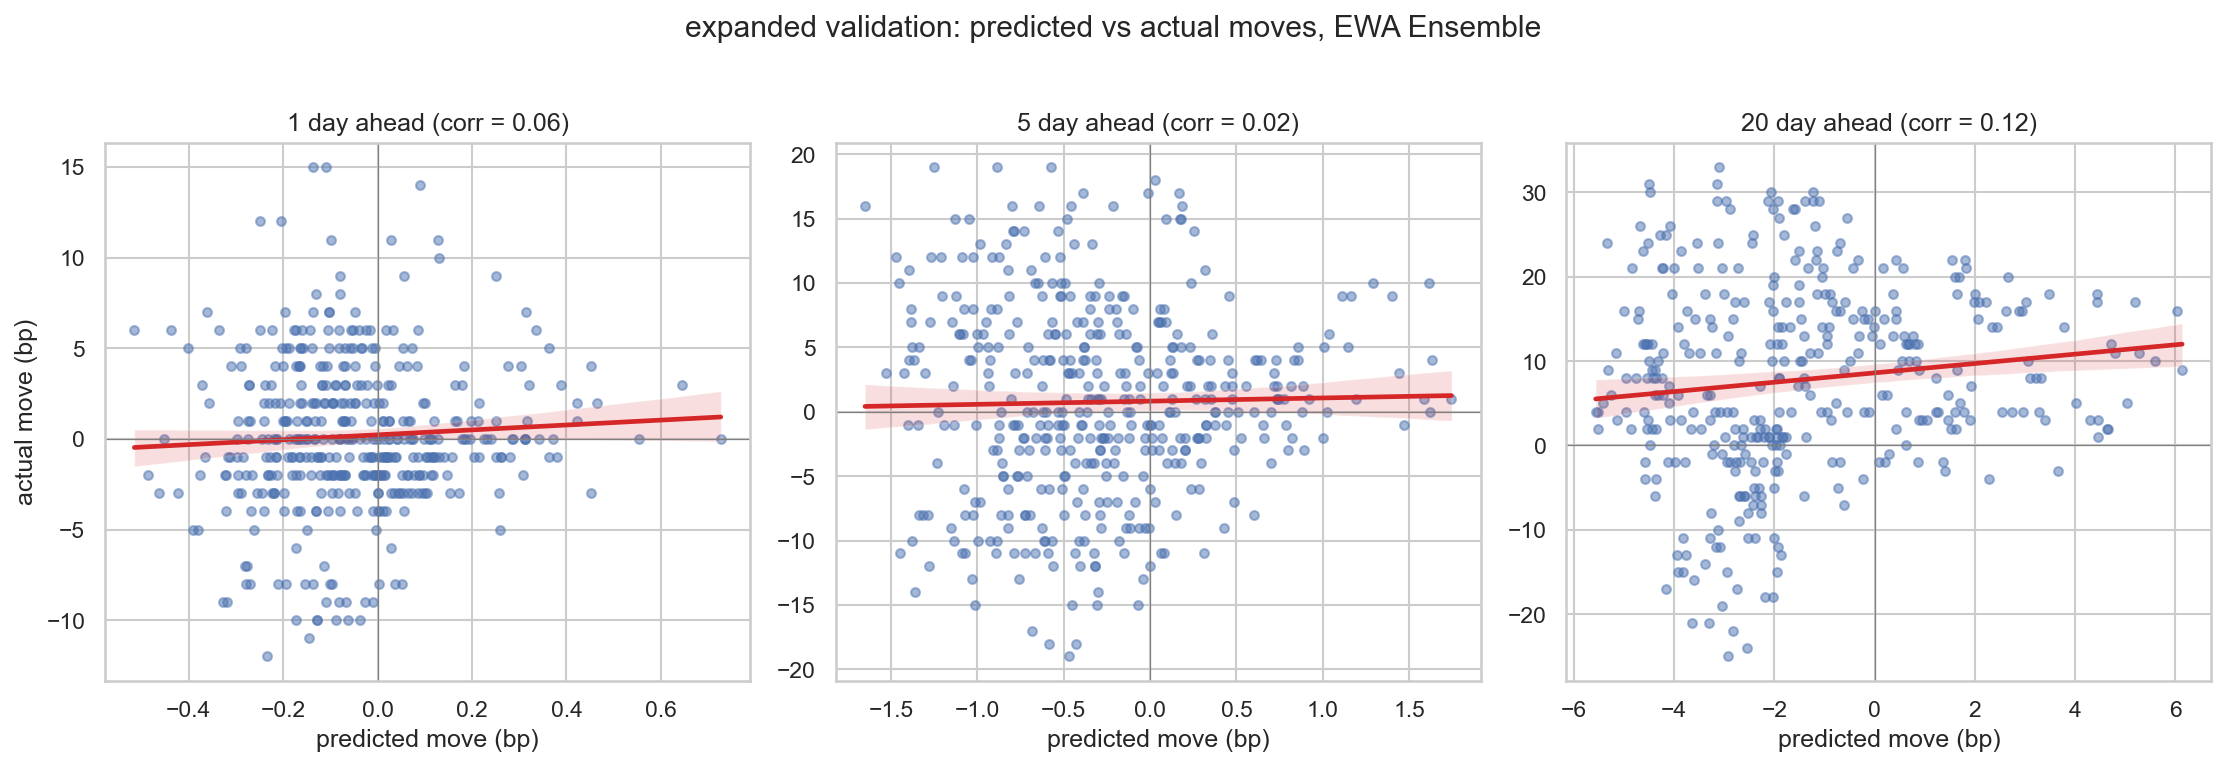
\includegraphics[width=0.98\textwidth]{validation_predicted_vs_actual_moves.png}
\caption{Validation on post-development data: predicted versus realized yield moves for the EWA ensemble by horizon, with fitted relationships. Correlations are 0.06, 0.02, and 0.12, reflecting the sharp July 2026 reversal that the adaptive system did not anticipate.}
\label{fig:forward}
\end{figure}

\section{Discussion}

Three lessons emerge. First, parameterization can dominate information. The identical feature set fails against the random walk when predicting levels and succeeds when predicting changes, because regularization determines what the model degrades into when the features are uninformative: a stale historical average in the first case, the strongest known benchmark in the second. The tuned configuration, an expanding window with a ridge penalty of 1{,}000, formalizes the resulting philosophy of a heavily shrunk tilt away from the random walk. Analogously, optimizing the decay parameter on training data rather than adopting the conventional month-unit value both improves the cross-sectional fit and makes the residual correction well defined.

Second, the predictive content of duration-aware regimes and spillover networks is real but conditional. It appears at horizons of five to twenty days, not at one day; it concentrates in trending policy regimes, as the 2022 results and the combination-weight path show; and it manifests more strongly in directional and size-weighted criteria than in RMSE, where improvements are approximately one basis point at twenty days. A companion experiment that replaced the regime and network features with literature-motivated economic features (multi-scale momentum, post-announcement drift, and policy-rate anchoring) performed worse on identical windows, with error correlations of 0.96 to 0.99 against the present specification, indicating that the regime, network, and lag features already span that information.

Third, honest evaluation changes conclusions. Naive directional accuracy scores the random walk near zero because it predicts no change, flattering every alternative; excluding unscorable observations and reporting base rates removes the illusion. Twenty-one-window evaluations of the kind common in exploratory work contain roughly one independent twenty-day observation and cannot support inference; the present design uses 1{,}149 windows and still treats one-day results as inconclusive. All reported p-values are conditional on the specification search that produced the final model, a fact we state rather than obscure, and the forward test exists precisely to provide evidence free of that conditioning.

Limitations include the equal-notional trading construction, which ignores duration risk differences across maturities; stylized transaction costs; the limited validation window, bounded by the availability of the macro series; and the treatment of same-day macro inputs as observable at the close, which a live implementation should lag by one day.

\section{Future Work}

Five directions follow naturally from these results. First, continued forward collection is the highest-priority item: the validation sample is bounded by the availability of the breakeven and policy-rate series, and refreshing those inputs as they are released extends the unconditioned sample with no methodological changes. A pre-registered protocol, freezing the specification, recording forecasts before outcomes are observed, and committing to report results regardless of direction, would make the accumulating evidence fully auditable.

Second, the July 2026 reversal identifies the system's principal weakness, and two remedies are testable within the existing framework. The combination weight could be conditioned on the filtered regime state, so that trust in the trend-following component is granted separately within each regime rather than pooled across them, and the loss discount could be shortened when filtered regime probabilities move abruptly, allowing faster retreat to the benchmark when conditions change.

Third, the trading evaluation can be moved toward implementability: netting positions across overlapping horizons to reduce turnover, applying tenor-specific futures transaction costs rather than a uniform charge, and weighting positions by duration risk rather than equal notional. Preliminary experiments during development suggested that turnover netting substantially reduces cost drag; a systematic treatment is warranted.

Fourth, the feature set could be extended with information sources that are genuinely exogenous to the yield history, most notably the Treasury auction calendar and auction outcome statistics, which are freely available and have documented local effects on yields near issuance dates. Care is required, as this study's experience with literature-motivated features shows that information already spanned by the factor, regime, and network variables adds nothing.

Fifth, the inference toolkit could be completed with a model confidence set analysis alongside the reality check, and the framework could be applied to other sovereign curves, where different policy regimes and market structures would test whether the regime-conditional pattern documented here generalizes.

\section{Conclusion}

Duration-aware regime features and cross-maturity spillover measures improve dynamic Nelson-Siegel forecasts of the Treasury curve by margins that are small in RMSE, meaningful in direction, and concentrated at the twenty-day horizon and in trending policy regimes. The enabling methodology is as important as the features: a training-optimized decay parameter, causally filtered regime probabilities, change-space targets that make regularization shrink toward the random walk, a per-maturity residual correction, and an adaptive combination with the benchmark. Under a profitability criterion with a signal threshold and trading costs, the system captures 28.2 percent of available basis-point movement at twenty days on more than a thousand evaluation windows. A small post-development validation sample containing a sharp July 2026 reversal shows the opposite sign, reinforcing that the edge is conditional on sustained trends and that continued forward collection is required before deployment claims. The one-day horizon, by contrast, offers no reliable signal to any model considered, and we caution against its use as a headline benchmark for yield-curve forecasting systems.

\section*{Acknowledgements}
The author thanks Dr. Christof Teuscher and the altREU program at Portland State University for guidance and support throughout this project.

\begin{thebibliography}{9}
\bibitem{diebold2006} Diebold, F.X., Li, C.: Forecasting the term structure of government bond yields. Journal of Econometrics 130(2), 337--364 (2006)
\bibitem{nelsonsiegel1987} Nelson, C.R., Siegel, A.F.: Parsimonious modeling of yield curves. Journal of Business 60(4), 473--489 (1987)
\bibitem{hamilton1989} Hamilton, J.D.: A new approach to the economic analysis of nonstationary time series and the business cycle. Econometrica 57(2), 357--384 (1989)
\bibitem{yu2010} Yu, S.-Z.: Hidden semi-Markov models. Artificial Intelligence 174(2), 215--243 (2010)
\bibitem{dieboldyilmaz2012} Diebold, F.X., Yilmaz, K.: Better to give than to receive: Predictive directional measurement of volatility spillovers. International Journal of Forecasting 28(1), 57--66 (2012)
\bibitem{pesaranshin1998} Pesaran, H.H., Shin, Y.: Generalized impulse response analysis in linear multivariate models. Economics Letters 58(1), 17--29 (1998)
\bibitem{dieboldmariano1995} Diebold, F.X., Mariano, R.S.: Comparing predictive accuracy. Journal of Business and Economic Statistics 13(3), 253--263 (1995)
\bibitem{harvey1997} Harvey, D., Leybourne, S., Newbold, P.: Testing the equality of prediction mean squared errors. International Journal of Forecasting 13(2), 281--291 (1997)
\bibitem{benjamini1995} Benjamini, Y., Hochberg, Y.: Controlling the false discovery rate: A practical and powerful approach to multiple testing. Journal of the Royal Statistical Society, Series B 57(1), 289--300 (1995)
\bibitem{hansen2005} Hansen, P.R.: A test for superior predictive ability. Journal of Business and Economic Statistics 23(4), 365--380 (2005)
\bibitem{politisromano1994} Politis, D.N., Romano, J.P.: The stationary bootstrap. Journal of the American Statistical Association 89(428), 1303--1313 (1994)
\bibitem{cesabianchi2006} Cesa-Bianchi, N., Lugosi, G.: Prediction, Learning, and Games. Cambridge University Press, Cambridge (2006)
\bibitem{duffee2013} Duffee, G.R.: Forecasting interest rates. In: Elliott, G., Timmermann, A. (eds.) Handbook of Economic Forecasting, vol. 2A, pp. 385--426. Elsevier, Amsterdam (2013)
\bibitem{koopman2010} Koopman, S.J., Mallee, M.I.P., Van der Wel, M.: Analyzing the term structure of interest rates using the dynamic Nelson-Siegel model with time-varying parameters. Journal of Business and Economic Statistics 28(3), 329--343 (2010)
\bibitem{litterman1991} Litterman, R., Scheinkman, J.: Common factors affecting bond returns. Journal of Fixed Income 1(1), 54--61 (1991)
\bibitem{ferguson1980} Ferguson, J.D.: Variable duration models for speech. In: Proceedings of the Symposium on the Application of Hidden Markov Models to Text and Speech, pp. 143--179 (1980)
\bibitem{bulla2006} Bulla, J., Bulla, I.: Stylized facts of financial time series and hidden semi-Markov models. Computational Statistics and Data Analysis 51(4), 2192--2209 (2006)
\bibitem{dieboldyilmaz2014} Diebold, F.X., Yilmaz, K.: On the network topology of variance decompositions: Measuring the connectedness of financial firms. Journal of Econometrics 182(1), 119--134 (2014)
\bibitem{hoerl1970} Hoerl, A.E., Kennard, R.W.: Ridge regression: Biased estimation for nonorthogonal problems. Technometrics 12(1), 55--67 (1970)
\bibitem{batesgranger1969} Bates, J.M., Granger, C.W.J.: The combination of forecasts. Operational Research Quarterly 20(4), 451--468 (1969)
\bibitem{timmermann2006} Timmermann, A.: Forecast combinations. In: Elliott, G., Granger, C.W.J., Timmermann, A. (eds.) Handbook of Economic Forecasting, vol. 1, pp. 135--196. Elsevier, Amsterdam (2006)
\bibitem{white2000} White, H.: A reality check for data snooping. Econometrica 68(5), 1097--1126 (2000)
\end{thebibliography}

\end{document}
